%% This file was auto-generated by IPython.
%% Conversion from the original notebook file:
%% meanshift.ipynb
%%
\documentclass[11pt,english,fleqn]{article}

%% This is the automatic preamble used by IPython.  Note that it does *not*
%% include a documentclass declaration, that is added at runtime to the overall
%% document.

\usepackage{amsmath}
\usepackage{amssymb}
\usepackage{graphicx}
\usepackage{ucs}
\usepackage[utf8x]{inputenc}

% needed for markdown enumerations to work
\usepackage{enumerate}

% Slightly bigger margins than the latex defaults
\usepackage{geometry}
\geometry{verbose,tmargin=3cm,bmargin=3cm,lmargin=2.5cm,rmargin=2.5cm}

% Define a few colors for use in code, links and cell shading
\usepackage{color}
\definecolor{orange}{cmyk}{0,0.4,0.8,0.2}
\definecolor{darkorange}{rgb}{.71,0.21,0.01}
\definecolor{darkgreen}{rgb}{.12,.54,.11}
\definecolor{myteal}{rgb}{.26, .44, .56}
\definecolor{gray}{gray}{0.45}
\definecolor{lightgray}{gray}{.95}
\definecolor{mediumgray}{gray}{.8}
\definecolor{inputbackground}{rgb}{.95, .95, .85}
\definecolor{outputbackground}{rgb}{.95, .95, .95}
\definecolor{traceback}{rgb}{1, .95, .95}

% Framed environments for code cells (inputs, outputs, errors, ...).  The
% various uses of \unskip (or not) at the end were fine-tuned by hand, so don't
% randomly change them unless you're sure of the effect it will have.
\usepackage{framed}

% remove extraneous vertical space in boxes
\setlength\fboxsep{0pt}

% codecell is the whole input+output set of blocks that a Code cell can
% generate.

% TODO: unfortunately, it seems that using a framed codecell environment breaks
% the ability of the frames inside of it to be broken across pages.  This
% causes at least the problem of having lots of empty space at the bottom of
% pages as new frames are moved to the next page, and if a single frame is too
% long to fit on a page, will completely stop latex from compiling the
% document.  So unless we figure out a solution to this, we'll have to instead
% leave the codecell env. as empty.  I'm keeping the original codecell
% definition here (a thin vertical bar) for reference, in case we find a
% solution to the page break issue.

%% \newenvironment{codecell}{%
%%     \def\FrameCommand{\color{mediumgray} \vrule width 1pt \hspace{5pt}}%
%%    \MakeFramed{\vspace{-0.5em}}}
%%  {\unskip\endMakeFramed}

% For now, make this a no-op...
\newenvironment{codecell}{}

 \newenvironment{codeinput}{%
   \def\FrameCommand{\colorbox{inputbackground}}%
   \MakeFramed{\advance\hsize-\width \FrameRestore}}
 {\unskip\endMakeFramed}

\newenvironment{codeoutput}{%
   \def\FrameCommand{\colorbox{outputbackground}}%
   \vspace{-1.4em}
   \MakeFramed{\advance\hsize-\width \FrameRestore}}
 {\unskip\medskip\endMakeFramed}

\newenvironment{traceback}{%
   \def\FrameCommand{\colorbox{traceback}}%
   \MakeFramed{\advance\hsize-\width \FrameRestore}}
 {\endMakeFramed}

% Use and configure listings package for nicely formatted code
\usepackage{listingsutf8}
\lstset{
  language=python,
  inputencoding=utf8x,
  extendedchars=\true,
  aboveskip=\smallskipamount,
  belowskip=\smallskipamount,
  xleftmargin=2mm,
  breaklines=true,
  basicstyle=\small \ttfamily,
  showstringspaces=false,
  keywordstyle=\color{blue}\bfseries,
  commentstyle=\color{myteal},
  stringstyle=\color{darkgreen},
  identifierstyle=\color{darkorange},
  columns=fullflexible,  % tighter character kerning, like verb
}

% The hyperref package gives us a pdf with properly built
% internal navigation ('pdf bookmarks' for the table of contents,
% internal cross-reference links, web links for URLs, etc.)
\usepackage{hyperref}
\hypersetup{
  breaklinks=true,  % so long urls are correctly broken across lines
  colorlinks=true,
  urlcolor=blue,
  linkcolor=darkorange,
  citecolor=darkgreen,
  }

% hardcode size of all verbatim environments to be a bit smaller
\makeatletter 
\g@addto@macro\@verbatim\small\topsep=0.5em\partopsep=0pt
\makeatother 

% Prevent overflowing lines due to urls and other hard-to-break entities.
\sloppy

\setlength{\mathindent}{0pt}
\setlength{\parindent}{0pt}
\setlength{\parskip}{8pt}
\begin{document}

Ortalama Kaydirma ile Kumeleme (Mean Shift Clustering)

Kumeleme yapmak icin bir metot daha: Ortalama Kaydirma metotu. Bu
metodun mesela K-Means'den farki kume sayisinin onceden belirtilmeye
ihtiyaci ol\textbf{ma}masidir, kume sayisi otomatik olarak metot
tarafindan saptanir.

``Kume'' olarak saptanan aslinda veri icindeki tum yogunluk bolgelerinin
merkezleridir, yani alttaki resmin sag kismindaki bolgeler.

\begin{codecell}
\begin{codeinput}
\begin{lstlisting}
im=imread("dist.png"); imshow(im)
\end{lstlisting}
\end{codeinput}
\begin{codeoutput}
\begin{verbatim}
<matplotlib.image.AxesImage at 0xa3f3c4c>
\end{verbatim}
\begin{center}
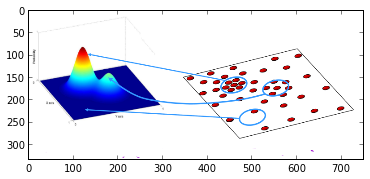
\includegraphics[width=0.7\textwidth]{meanshift_files/meanshift_fig_00.png}
\par
\end{center}
\end{codeoutput}
\end{codecell}
Baslangic neresidir? Baslangic tum noktalardir, yani her noktadan
baslanarak

\begin{enumerate}[1.]
\item
  O nokta etrafinda (yeterince buyuk) bir pencere tanimla
\item
  Bu pencere icine dusen tum noktalari hesaba katarak bir ortalama yer
  hesapla
\item
  Pencereyi yeni ortalama noktayi merkezine alacak sekilde kaydir
\end{enumerate}
Metotun ismi buradan geliyor, cunku pencere yeni ortalamaya dogru
``kaydiriliyor''. Altta bir noktadan baslanarak yapilan hareketi
goruyoruz. Kaymanin saga dogru olmasi mantikli cunku tek pencere icinden
bakinca bile yogunlugun ``sag tarafa dogru'' oldugu gorulmekte. Yontemin
puf noktasi burada.

\begin{codecell}
\begin{codeinput}
\begin{lstlisting}
im=imread("mean_2.png"); imshow(im)

\end{lstlisting}
\end{codeinput}
\begin{codeoutput}
\begin{verbatim}
<matplotlib.image.AxesImage at 0x9b966ac>
\end{verbatim}
\begin{center}
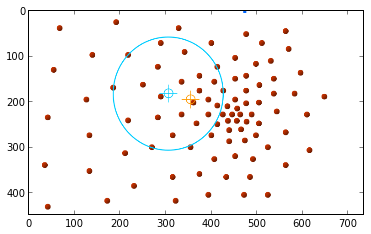
\includegraphics[width=0.7\textwidth]{meanshift_files/meanshift_fig_01.png}
\par
\end{center}
\end{codeoutput}
\end{codecell}
\begin{codecell}
\begin{codeinput}
\begin{lstlisting}
im=imread("mean_3.png"); imshow(im)

\end{lstlisting}
\end{codeinput}
\begin{codeoutput}
\begin{verbatim}
<matplotlib.image.AxesImage at 0x9cd99ec>
\end{verbatim}
\begin{center}
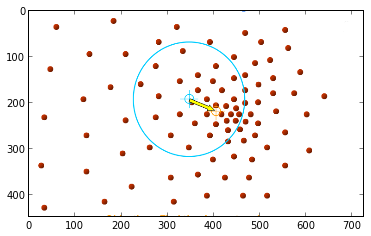
\includegraphics[width=0.7\textwidth]{meanshift_files/meanshift_fig_02.png}
\par
\end{center}
\end{codeoutput}
\end{codecell}
\begin{codecell}
\begin{codeinput}
\begin{lstlisting}
im=imread("mean_4.png"); imshow(im)

\end{lstlisting}
\end{codeinput}
\begin{codeoutput}
\begin{verbatim}
<matplotlib.image.AxesImage at 0x9e3cfac>
\end{verbatim}
\begin{center}
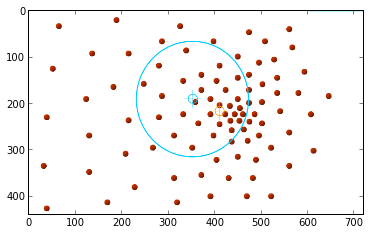
\includegraphics[width=0.7\textwidth]{meanshift_files/meanshift_fig_03.png}
\par
\end{center}
\end{codeoutput}
\end{codecell}
\begin{codecell}
\begin{codeinput}
\begin{lstlisting}
im=imread("mean_5.png"); imshow(im)

\end{lstlisting}
\end{codeinput}
\begin{codeoutput}
\begin{verbatim}
<matplotlib.image.AxesImage at 0x9f9b5ec>
\end{verbatim}
\begin{center}
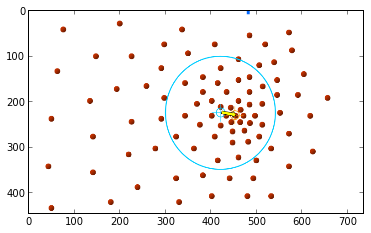
\includegraphics[width=0.7\textwidth]{meanshift_files/meanshift_fig_04.png}
\par
\end{center}
\end{codeoutput}
\end{codecell}
\begin{codecell}
\begin{codeinput}
\begin{lstlisting}
im=imread("mean_6.png"); imshow(im)

\end{lstlisting}
\end{codeinput}
\begin{codeoutput}
\begin{verbatim}
<matplotlib.image.AxesImage at 0xa13cd0c>
\end{verbatim}
\begin{center}
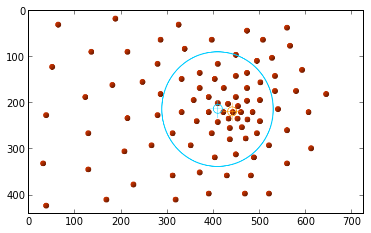
\includegraphics[width=0.7\textwidth]{meanshift_files/meanshift_fig_05.png}
\par
\end{center}
\end{codeoutput}
\end{codecell}
\begin{codecell}
\begin{codeinput}
\begin{lstlisting}
im=imread("mean_7.png"); imshow(im)

\end{lstlisting}
\end{codeinput}
\begin{codeoutput}
\begin{verbatim}
<matplotlib.image.AxesImage at 0xa2a132c>
\end{verbatim}
\begin{center}
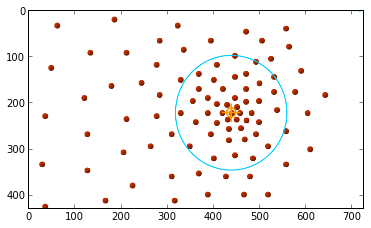
\includegraphics[width=0.7\textwidth]{meanshift_files/meanshift_fig_06.png}
\par
\end{center}
\end{codeoutput}
\end{codecell}
Eger yogunluk merkezine cok yakin bir noktadan / noktalardan baslamissak
ne olur?

O zaman ilerleme o baslangic noktasi icin aninda bitecek, cunku hemen
yogunluk merkezine gelmis olacagiz. Diger yonlerden gelen pencereler de
ayni yere gelecekler tabii, o zaman ayni / yakin yogunluk merkezlerini
ayni kume olarak kabul etmemiz gerekir. Bu ``ayni kume irdelemesi''
sayisal hesaplama acisindan ufak farklar gosterebilir tabii, ve bu ufak
farki gozonune alarak ``kume birlestirme'' mantigini da eklemek
gerekiyor.

Ortalama Kaydirma sisteminde pencere buyuklugu kullanici tarafindan
tanimlanir. Optimal pencere buyuklugunu nasil buluruz? Deneme yanilma
yontemi, verinin tarifsel istatistiklerine kestirme bir hesap (estimate)
etmek, ya da kullanicinin ayni istatistiklere bakarak tahminde
bulunmasi. Birkac farkli pencere buyuklugu de denenebilir. Bu konu
literaturde (Ing. bandwidth selection) adi atlinda uzun uzadiya
tartisilmaktadir. Fakat evet, kullanici tarafindan tanimli bu
parametrenin bir anlamda bu metotun bir zayifligi oldugu soylenebilir.
KMeans kume sayisini istiyordu, bu metot ta pencere buyuklugunu istiyor.
Hangi metotun ne zaman uygun oldugunu anlamak tecrube gerektiriyor.

\begin{codecell}
\begin{codeinput}
\begin{lstlisting}
im=imread("start.png"); imshow(im)

\end{lstlisting}
\end{codeinput}
\begin{codeoutput}
\begin{verbatim}
<matplotlib.image.AxesImage at 0x9af0f2c>
\end{verbatim}
\begin{center}
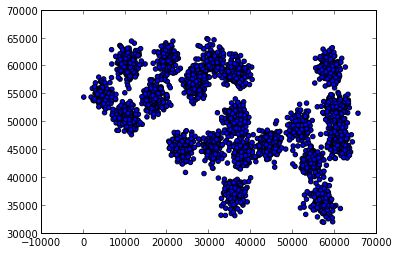
\includegraphics[width=0.7\textwidth]{meanshift_files/meanshift_fig_07.png}
\par
\end{center}
\end{codeoutput}
\end{codecell}
Altta ornek veri ve kodu bulabilirsiniz (kod scikit-learn adli
kutuphaneden alinmistir). Metot kume sayisi 17'yi otomatik olarak
buluyor.

Alternatif bir kod meanshift\_alternative.py dosyasinda bulunabilir, bu
kod pencereler kaydirirken onlarin uzerinden gectigi noktalari
``sahiplenen'' turden bir kod. Yani {[}encere hareketini durdurdugunda
hem kume merkezini hem de o kumenin altindaki noktalari bulmus oluyoruz.
Tabii sonraki pencereler bazi noktalari onceki kumelerden calabilirler.
Neyse, islemin normal isleyisine gore bir sonraki pencere secilecektir
ve bu pencere ``geriye kalan noktalar'' uzerinden islem yapacaktir.
Beklenir ki, islem ilerledikce islenmesi gereken noktalar azalacaktir ve
yontemin bu sebeple klasik yonteme gore daha hizli isleyecegi tahmin
edilebilir. Hakikaten de boyledir.

\begin{codecell}
\begin{codeinput}
\begin{lstlisting}
from pandas import *
data = read_csv("synthetic.txt",header=None,sep="   ")
print data.shape
data = np.array(data)
\end{lstlisting}
\end{codeinput}
\begin{codeoutput}
\begin{verbatim}
(3000, 2)
\end{verbatim}
\end{codeoutput}
\end{codecell}
\begin{codecell}
\begin{codeinput}
\begin{lstlisting}
scatter(data[:,0],data[:,1])
\end{lstlisting}
\end{codeinput}
\begin{codeoutput}
\begin{verbatim}
<matplotlib.collections.PathCollection at 0xa0b7e0c>
\end{verbatim}
\begin{center}
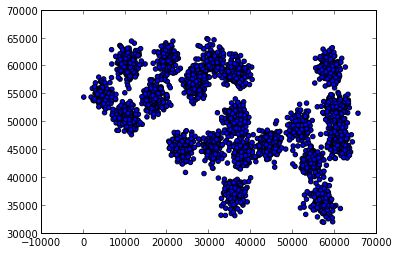
\includegraphics[width=0.7\textwidth]{meanshift_files/meanshift_fig_08.png}
\par
\end{center}
\end{codeoutput}
\end{codecell}
\begin{codecell}
\begin{codeinput}
\begin{lstlisting}
import numpy as np
from sklearn.neighbors import NearestNeighbors
from sklearn.utils import extmath

def mean_shift(X, bandwidth=None, max_iterations=300):
    
    seeds = X
    n_samples, n_features = X.shape
    stop_thresh = 1e-3 * bandwidth  # when mean has converged
    center_intensity_dict = {}
    nbrs = NearestNeighbors(radius=bandwidth).fit(X)

    # For each seed, climb gradient until convergence or max_iterations
    for my_mean in seeds:
        completed_iterations = 0
        while True:
            # Find mean of points within bandwidth
            i_nbrs = nbrs.radius_neighbors([my_mean], bandwidth,
                                           return_distance=False)[0]
            points_within = X[i_nbrs]
            if len(points_within) == 0:
                break  # Depending on seeding strategy this condition may occur
            my_old_mean = my_mean  # save the old mean
            my_mean = np.mean(points_within, axis=0)
            # If converged or at max_iterations, addS the cluster
            if (extmath.norm(my_mean - my_old_mean) < stop_thresh or
                    completed_iterations == max_iterations):
                center_intensity_dict[tuple(my_mean)] = len(points_within)
                break
            completed_iterations += 1

    # POST PROCESSING: remove near duplicate points
    # If the distance between two kernels is less than the bandwidth,
    # then we have to remove one because it is a duplicate. Remove the
    # one with fewer points.
    sorted_by_intensity = sorted(center_intensity_dict.items(),
                                 key=lambda tup: tup[1], reverse=True)
    sorted_centers = np.array([tup[0] for tup in sorted_by_intensity])
    unique = np.ones(len(sorted_centers), dtype=np.bool)
    nbrs = NearestNeighbors(radius=bandwidth).fit(sorted_centers)
    for i, center in enumerate(sorted_centers):
        if unique[i]:
            neighbor_idxs = nbrs.radius_neighbors([center],
                                                  return_distance=False)[0]
            unique[neighbor_idxs] = 0
            unique[i] = 1  # leave the current point as unique
    cluster_centers = sorted_centers[unique]

    # ASSIGN LABELS: a point belongs to the cluster that it is closest to
    nbrs = NearestNeighbors(n_neighbors=1).fit(cluster_centers)
    labels = np.zeros(n_samples, dtype=np.int)
    distances, idxs = nbrs.kneighbors(X)
    labels = idxs.flatten()
    
    return cluster_centers, labels
\end{lstlisting}
\end{codeinput}
\end{codecell}
\begin{codecell}
\begin{codeinput}
\begin{lstlisting}
cluster_centers, labels = mean_shift(np.array(data), 4000)

\end{lstlisting}
\end{codeinput}
\end{codecell}
\begin{codecell}
\begin{codeinput}
\begin{lstlisting}
print len(cluster_centers)
\end{lstlisting}
\end{codeinput}
\begin{codeoutput}
\begin{verbatim}
17
\end{verbatim}
\end{codeoutput}
\end{codecell}
\begin{codecell}
\begin{codeinput}
\begin{lstlisting}
scatter(data[:,0],data[:,1])
plt.hold(True)
for x in asarray(cluster_centers): plot(x[0],x[1],'rd')

\end{lstlisting}
\end{codeinput}
\begin{codeoutput}
\begin{center}
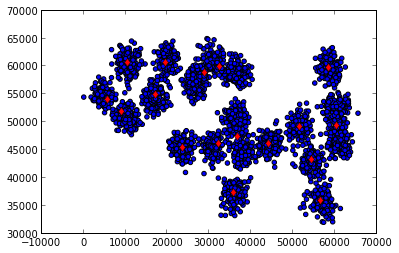
\includegraphics[width=0.7\textwidth]{meanshift_files/meanshift_fig_09.png}
\par
\end{center}
\end{codeoutput}
\end{codecell}
Teorik Konular

Bu metotu teorik bir yapiya oturtmak icin onu yazinin ilk basindaki
resimde oldugu gibi gormek gerekiyor, yani mesela o ilk resmin sagindaki
2 boyuttaki veri dagilimi (ki ayriksal, sayisal), 3 boyuttaki surekli
(continuous) bir baska dagilimin yansimasi sanki, ki o zaman 2 boyuttaki
yogunluk bolgeleri surekli dagilimdaki tepe noktalarini temsil
ediyorlar, ve biz o surekli versiyondaki tepe noktalarini bulmaliyiz.
Fakat kumeleme isleminin elinde sadece 2 boyuttaki veriler var, o zaman
surekli dagilimi bir sekilde yaratmak lazim.

Bunu yapmak icin problem / veri once bir Cekirdek Yogunluk Kestirimi
(Kernel Density Estimation -KDE-) problemi gibi goruluyor, ki her nokta
uzerine bir cekirdek fonksiyonu koyularak ve onlarin toplamim alinarak
sayisal dagilim puruzsuz bir hale getiriliyor. Ortalama Kaydirma icin
gerekli kayma ``yonu'' ise iste bu yeni surekli fonksiyonun gradyanidir
deniyor (elimizde bir surekli fonksiyon oldugu icin turev rahatlikla
alabiliyoruz), ve gradyan yerel tepe noktasini gosterdigi icin o yone
yapilan hareket bizi yavas yavas tepeye goturecektir. Bu hareketin yerel
tepeleri bulacagi, ve tum yontemin nihai olarak sonuca yaklasacagi
(convergence) matematiksel olarak ispat edilebilir.

KDE ile elde edilen teorik dagilim fonksiyonunun icbukey olup olmadigi
onemli degil (ki mesela lojistik regresyonda bu onemliydi), cunku nihai
tepe noktasini degil, birkac yerel tepe noktasindan birini (hatta
hepsini) bulmakla ilgileniyoruz. Gradyan bizi bu noktaya tasiyacaktir.

Kaynaklar

http://www.serc.iisc.ernet.in/\ensuremath{\sim}venky/SE263/slides/Mean-Shift-Theory.pdf

http://saravananthirumuruganathan.wordpress.com/2010/04/01/introduction-to-mean-shift-algorithm/

http://www.cse.yorku.ca/\ensuremath{\sim}kosta/CompVis\_Notes/mean\_shift.pdf

http://homepages.inf.ed.ac.uk/rbf/CVonline/LOCAL\_COPIES/TUZEL1/MeanShift.pdf

Scikit-Learn Kodlari

http://yotamgingold.com/code/MeanShiftCluster.py

\end{document}
